\documentclass[12pt,a4paper]{article}
\usepackage{ctex}
\usepackage{amsmath,amscd,amsbsy,amssymb,latexsym,url,bm,amsthm}
\usepackage{epsfig,graphicx,subfigure}
\usepackage{enumitem,balance}
\usepackage{wrapfig}
\usepackage{mathrsfs,euscript}
\usepackage[usenames]{xcolor}
\usepackage{hyperref}
\usepackage[vlined,ruled,linesnumbered]{algorithm2e}
\usepackage{array}
\hypersetup{colorlinks=true,linkcolor=black}

\newtheorem{theorem}{Theorem}
\newtheorem{lemma}[theorem]{Lemma}
\newtheorem{proposition}[theorem]{Proposition}
\newtheorem{corollary}[theorem]{Corollary}
\newtheorem{exercise}{Exercise}
\newtheorem*{solution}{Solution}
\newtheorem{definition}{Definition}
\theoremstyle{definition}

\renewcommand{\thefootnote}{\fnsymbol{footnote}}

\newcommand{\postscript}[2]
 {\setlength{\epsfxsize}{#2\hsize}
  \centerline{\epsfbox{#1}}}

\renewcommand{\baselinestretch}{1.0}

\setlength{\oddsidemargin}{-0.365in}
\setlength{\evensidemargin}{-0.365in}
\setlength{\topmargin}{-0.3in}
\setlength{\headheight}{0in}
\setlength{\headsep}{0in}
\setlength{\textheight}{10.1in}
\setlength{\textwidth}{7in}
\makeatletter \renewenvironment{proof}[1][Proof] {\par\pushQED{\qed}\normalfont\topsep6\p@\@plus6\p@\relax\trivlist\item[\hskip\labelsep\bfseries#1\@addpunct{.}]\ignorespaces}{\popQED\endtrivlist\@endpefalse} \makeatother
\makeatletter
\renewenvironment{solution}[1][Solution] {\par\pushQED{\qed}\normalfont\topsep6\p@\@plus6\p@\relax\trivlist\item[\hskip\labelsep\bfseries#1\@addpunct{.}]\ignorespaces}{\popQED\endtrivlist\@endpefalse} \makeatother

\begin{document}
\noindent

%========================================================================
\noindent\framebox[\linewidth]{\shortstack[c]{
\Large{\textbf{Lab10-Turing Machine}}\vspace{1mm}\\
CS214-Algorithm and Complexity, Xiaofeng Gao \& Lei Wang, Spring 2021.}}
\begin{center}
\footnotesize{\color{red}$*$ If there is any problem, please contact TA Yihao Xie. }

\footnotesize{\color{blue}$*$ Name:\underline{Xin Xu}  \quad Student ID:\underline{519021910726} \quad Email: \underline{xuxin20010203@sjtu.edu.cn}}
\end{center}

\begin{enumerate}
    \item Design a one-tape TM $M$ that computes the function $f(x, y) = \lfloor x/y \rfloor$, where $x$ and $y$ are positive integers $(x > y)$. The alphabet is $\{1, 0, \Box, \triangleright, \triangleleft\}$, and the inputs are $x$ "1"s, $\Box$ and $y$ "1"s. Below is the initial configuration for input $x=7$ and $y=3$. The result $z=f(x,y)$ should also be represented in the form of $z$ "1"s on the tape with pattern of $\rhd 111\cdots 111\lhd$, which is $\rhd 11\lhd$ for the example.
    
	\begin{center}
		\begin{tabular}{ll|c|c|c|c|c|c|c|c|c|c|c|c|c|c}
			& \multicolumn{14}{c}{Initial Configuration}\\[5pt]
			\cline{2-16}
			& & $\triangleright$ &  1  & 1 & 1 & 1 & 1 & 1 & 1 & $\Box$ & 1 & 1 & 1 & $ \triangleleft$ & \\
			\cline{2-16}
			\multicolumn{2}{c}{} & \multicolumn{1}{c}{$\uparrow$} & \multicolumn{11}{c}{}\\
			\multicolumn{2}{c}{} & \multicolumn{1}{c}{$q_S$} & \multicolumn{11}{c}{}	
		\end{tabular}
	\end{center}

    \begin{enumerate}
	\item
	Please describe your design and then write the specifications of $M$ in the form like $\langle q_S, \triangleright \rangle \rightarrow \langle q_1, \triangleright,  R\rangle$. Explain the transition functions in detail.
	
	\item
	Please draw the state transition diagram.
	
	\item
	Show briefly and clearly the whole process from initial to final configurations for input $x = 7$ and $y = 3$. You may start like this:
	$$(q_s,\underline{\triangleright}  1  1  1  1  1  1  1  \Box 1  1  1   \triangleleft)
	\vdash (q_1,\triangleright  \underline{1}  1  1  1  1  1  1  \Box 1  1  1   \triangleleft)
	\vdash^* (q_1,\triangleright  1  1  1  1  1  1  1  \underline{\Box} 1  1  1   \triangleleft)
	\vdash (q_2,\triangleright  1  1  1  1  1  1  1  \Box \underline{1}  1  1   \triangleleft)$$
	
	\par{\color{blue}(Note that for simplicity, we write $(q_1,\triangleright  \underline{1}  1  1  1  1  1  1  \Box 1  1  1   \triangleleft)\vdash^* (q_1,\triangleright  1  1  1  1  1  1  1  \underline{\Box} 1  1  1   \triangleleft)$ if the corresponding transaction repeats on multiple inputs with the same state.)}
	
\end{enumerate}

    \begin{solution}
		\begin{enumerate}
			\item My design is to transfer $x,y$ "1" to "0" everytime encountering $y$ "1" and add "1" when encountering $\triangleright$. The specifications are below:\\
			$\langle q_S, \triangleright \rangle \rightarrow \langle q_1, \triangleright,  R\rangle$\\
			$\langle q_1, 1 \rangle \rightarrow \langle q_1, 1,  R\rangle$\\
			$\langle q_1, \triangleleft \rangle \rightarrow \langle q_1, \triangleleft,  R\rangle$\\
			$\langle q_1, 0 \rangle \rightarrow \langle q_1, 0,  R\rangle$\\
			$\langle q_1, \Box \rangle \rightarrow \langle q_2, \Box,  R\rangle$\\
			$q_1$ is used to go right and across $\Box$. After acrossing, the state becomes $q_2$.\\
			$\langle q_2, 0 \rangle \rightarrow \langle q_2, 0,  R\rangle$\\
			$\langle q_2, 1 \rangle \rightarrow \langle q_3, 0,  L\rangle$\\
			$\langle q_2, \triangleleft \rangle \rightarrow \langle q_w, \triangleleft,  L\rangle$\\
			$q_2$ is used to change 1 to 0 so that after all 1 in $y$ has to be changed, the quotient can increase by 1.\\
			$\langle q_3, 0 \rangle \rightarrow \langle q_3, 0,  L\rangle$\\
			$\langle q_3, 1 \rangle \rightarrow \langle q_3, 1,  L\rangle$\\
			$\langle q_3, \Box \rangle \rightarrow \langle q_4, \Box,  L\rangle$\\
			$q_3$ is used to go left and across $\Box$. After acrossing, the state becomes $q_4$.\\
			$\langle q_4, 1 \rangle \rightarrow \langle q_1, 0,  R\rangle$\\
			$\langle q_4, 0 \rangle \rightarrow \langle q_4, 0,  L\rangle$\\
			$\langle q_4, \triangleleft \rangle \rightarrow \langle q_4, \triangleleft,  L\rangle$\\
			$\langle q_4, \triangleright \rangle \rightarrow \langle q_c, \triangleright,  R\rangle$\\
			$q_4$ is used to change 1 to 0 in $x$.\\
			$\langle q_w, 0 \rangle \rightarrow \langle q_w, 0,  L\rangle$\\
			$\langle q_w, \Box \rangle \rightarrow \langle q_d, \Box,  L\rangle$\\
			$q_w$ is used to go left and across $\Box$. After acrossing, the state becomes $q_d$.\\
			$\langle q_d, 0 \rangle \rightarrow \langle q_b, \triangleleft,  R\rangle$\\
			$\langle q_d, \triangleleft \rangle \rightarrow \langle q_d, \triangleleft,  L\rangle$\\
			$q_d$ is used to increase the quotient. The number of $\triangleleft $ by the left of $\Box$ is the quotient.\\
			$\langle q_b, \triangleleft \rangle \rightarrow \langle q_b, \triangleleft,  R\rangle$\\
			$\langle q_b, \Box \rangle \rightarrow \langle q_f, \Box,  R\rangle$\\
			$\langle q_f, 0 \rangle \rightarrow \langle q_f, 1,  R\rangle$\\
			$\langle q_f, \triangleleft \rangle \rightarrow \langle q_f, \triangleleft,  L\rangle$\\
			$\langle q_f, 1 \rangle \rightarrow \langle q_f, 1,  L\rangle$\\
			$\langle q_f, \Box \rangle \rightarrow \langle q_2, \Box,  R\rangle$\\
			$q_b$ and $q_f$ are used to regain the divisor. $q_b$ is used to go right and $q_f$ is used to regain.\\
			$\langle q_c, 0 \rangle \rightarrow \langle q_c, 0,  R\rangle$\\
			$\langle q_c, \triangleleft \rangle \rightarrow \langle q_c, 1,  R\rangle$\\
			$\langle q_c, \Box \rangle \rightarrow \langle q_p, 0,  R\rangle$\\
			$\langle q_p, 1 \rangle \rightarrow \langle q_p, 0,  R\rangle$\\
			$\langle q_p, \triangleleft \rangle \rightarrow \langle q_H, \triangleleft,  S\rangle$\\
			$q_c$ and $q_p$ are used to transfer $\triangleleft$ to 1 and transfer other symbols to 0 and finally terminate the machine.
			\item The diagram is below:\\
			\begin{figure}[!htbp]
				\centering
				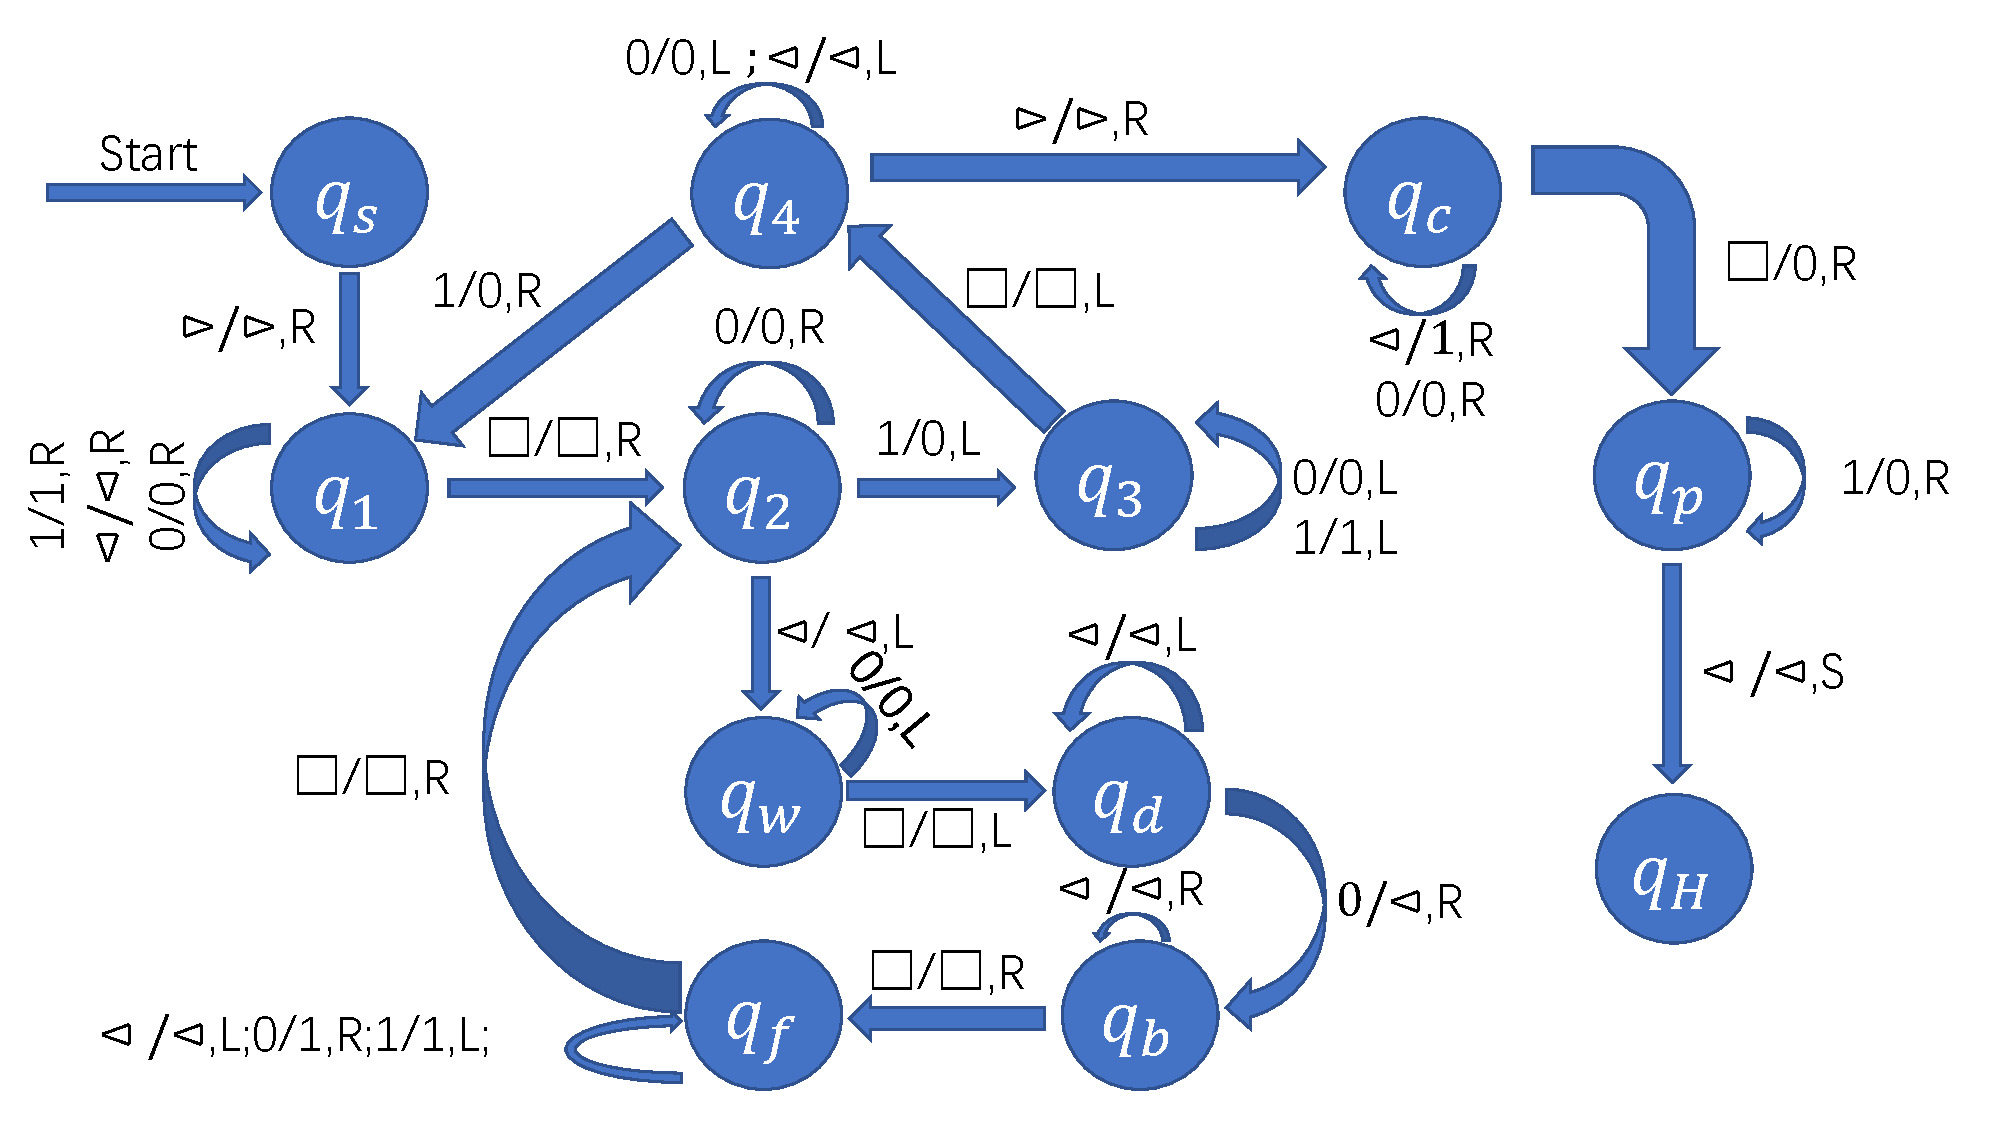
\includegraphics[width=0.5\textwidth]{Transition diagram.pdf}
				\caption{The transition diagram of the one type TM}
				\label{Fig-Diagram}
			\end{figure}
			\item $$(q_s,\underline{\triangleright}  1  1  1  1  1  1  1  \Box 1  1  1   \triangleleft)
			\vdash (q_1,\triangleright  \underline{1}  1  1  1  1  1  1  \Box 1  1  1   \triangleleft)
			\vdash^* (q_1,\triangleright  1  1  1  1  1  1  1  \underline{\Box} 1  1  1   \triangleleft)
			\vdash (q_2,\triangleright  1  1  1  1  1  1  1  \Box \underline{1}  1  1   \triangleleft)$$
			$$\vdash (q_3,\triangleright  1  1  1  1  1  1  1  \underline{\Box} 0  1  1   \triangleleft)
			\vdash (q_4,\triangleright  1  1  1  1  1  1  \underline{1}  \Box 0  1  1   \triangleleft)
			\vdash (q_1,\triangleright  1  1  1  1  1  1  0  \underline{\Box} 0  1  1   \triangleleft)
			\vdash (q_2,\triangleright  1  1  1  1  1  1  0  \Box \underline{0}  1  1   \triangleleft)$$
			$$\vdash (q_2,\triangleright  1  1  1  1  1  1  0  \Box 0  \underline{1}  1   \triangleleft)
			\vdash (q_3,\triangleright  1  1  1  1  1  1  0  \underline{\Box} 0  0  1   \triangleleft)
			\vdash (q_4,\triangleright  1  1  1  1  1  1  \underline{0}  \Box 0  0  1   \triangleleft)
			\vdash (q_4,\triangleright  1  1  1  1  1  \underline{1}  0  \Box 0  0  1   \triangleleft)$$
			$$\vdash (q_1,\triangleright  1  1  1  1  1  0  0  \underline{\Box} 0  0  1   \triangleleft)
			\vdash (q_2,\triangleright  1  1  1  1  1  0  0  \Box \underline{0}  0  1   \triangleleft)
			\vdash (q_2,\triangleright  1  1  1  1  1  0  0  \Box 0  0  \underline{1}   \triangleleft)
			\vdash (q_3,\triangleright  1  1  1  1  1  0  0  \underline{\Box} 0  0  0   \triangleleft)$$
			$$\vdash (q_4,\triangleright  1  1  1  1  1  0  \underline{0}  \Box 0  0  0   \triangleleft)
			\vdash (q_4,\triangleright  1  1  1  1  \underline{1}  0  0  \Box 0  0  0   \triangleleft)
			\vdash (q_1,\triangleright  1  1  1  1  0  0  0  \underline{\Box} 0  0  0   \triangleleft)
			\vdash (q_2,\triangleright  1  1  1  1  0  0  0  \Box \underline{0}  0  0   \triangleleft)$$
			$$\vdash (q_2,\triangleright  1  1  1  1  0  0  0  \Box 0  0  0   \underline{\triangleleft})
			\vdash (q_w,\triangleright  1  1  1  1  0  0  0  \Box 0  0  \underline{0}   \triangleleft)
			\vdash (q_w,\triangleright  1  1  1  1  0  0  0  \underline{\Box} 0  0  0   \triangleleft)
			\vdash (q_d,\triangleright  1  1  1  1  0  0  \underline{0}  \Box 0  0  0   \triangleleft)$$
			$$\vdash (q_b,\triangleright  1  1  1  1  0  0  \triangleleft  \underline{\Box} 0  0  0   \triangleleft)
			\vdash (q_f,\triangleright  1  1  1  1  0  0  \triangleleft  \Box \underline{0}  0  0   \triangleleft)
			\vdash (q_f,\triangleright  1  1  1  1  0  0  \triangleleft  \Box 1  \underline{0}  0   \triangleleft)
			\vdash (q_f,\triangleright  1  1  1  1  0  0  \triangleleft  \Box 1  1  \underline{0}   \triangleleft)$$
			$$\vdash (q_f,\triangleright  1  1  1  1  0  0  \triangleleft  \Box 1  1  1   \underline{\triangleleft})
			\vdash (q_f,\triangleright  1  1  1  1  0  0  \triangleleft  \underline{\Box} 1  1  1   \triangleleft)
			\vdash (q_2,\triangleright  1  1  1  1  0  0  \triangleleft  \Box \underline{1}  1  1   \triangleleft)
			\vdash (q_3,\triangleright  1  1  1  1  0  0  \triangleleft  \underline{\Box} 0  1  1   \triangleleft)$$
			$$\vdash (q_4,\triangleright  1  1  1  1  0  0  \underline{\triangleleft}  \Box 0  1  1   \triangleleft)
			\vdash (q_4,\triangleright  1  1  1  1  0  \underline{0}  \triangleleft  \Box 0  1  1   \triangleleft)
			\vdash (q_4,\triangleright  1  1  1  \underline{1}  0  0  \triangleleft  \Box 0  1  1   \triangleleft)
			\vdash (q_1,\triangleright  1  1  1  0  0  0  \triangleleft  \underline{\Box} 0  1  1   \triangleleft)$$
			$$\vdash (q_2,\triangleright  1  1  1  0  0  0  \triangleleft  \Box \underline{0}  1  1   \triangleleft)
			\vdash (q_2,\triangleright  1  1  1  0  0  0  \triangleleft  \Box 0  \underline{1}  1   \triangleleft)
			\vdash (q_3,\triangleright  1  1  1  0  0  0  \triangleleft  \underline{\Box} 0  0  1   \triangleleft)
			\vdash (q_4,\triangleright  1  1  1  0  0  0  \underline{\triangleleft}  \Box 0  0  1   \triangleleft)$$
			$$\vdash (q_4,\triangleright  1  1  \underline{1}  0  0  0  \triangleleft  \Box 0  0  1   \triangleleft)
			\vdash (q_1,\triangleright  1  1  0  0  0  0  \triangleleft  \underline{\Box} 0  0  1   \triangleleft)
			\vdash (q_2,\triangleright  1  1  0  0  0  0  \triangleleft  \Box \underline{0}  0  1   \triangleleft)
			\vdash (q_2,\triangleright  1  1  0  0  0  0  \triangleleft  \Box 0  0  \underline{1}   \triangleleft)$$
			$$\vdash (q_3,\triangleright  1  1  0  0  0  0  \triangleleft  \underline{\Box} 0  0  0   \triangleleft)
			\vdash (q_4,\triangleright  1  1  0  0  0  0  \underline{\triangleleft}  \Box 0  0  0   \triangleleft)
			\vdash (q_4,\triangleright  1  \underline{1}  0  0  0  0  \triangleleft  \Box 0  0  0   \triangleleft)
			\vdash (q_1,\triangleright  1  0  0  0  0  0  \triangleleft  \underline{\Box} 0  0  0   \triangleleft)$$
			$$\vdash (q_2,\triangleright  1  0  0  0  0  0  \triangleleft  \Box \underline{0}  0  0   \triangleleft)
			\vdash (q_2,\triangleright  1  0  0  0  0  0  \triangleleft  \Box 0  0  0   \underline{\triangleleft})
			\vdash (q_w,\triangleright  1  0  0  0  0  0  \triangleleft  \Box 0  0  \underline{0}   \triangleleft)
			\vdash (q_w,\triangleright  1  0  0  0  0  0  \triangleleft  \underline{\Box} 0  0  0   \triangleleft)$$
            $$\vdash (q_d,\triangleright  1  0  0  0  0  0  \underline{\triangleleft}  \Box 0  0  0   \triangleleft)
			\vdash (q_d,\triangleright  1  0  0  0  0  \underline{0}  \triangleleft  \Box 0  0  0   \triangleleft)
			\vdash (q_b,\triangleright  1  0  0  0  0  \triangleleft  \triangleleft  \underline{\Box} 0  0  0   \triangleleft)
			\vdash (q_f,\triangleright  1  0  0  0  0  \triangleleft  \triangleleft  \Box \underline{0}  0  0   \triangleleft)$$
			$$\vdash (q_f,\triangleright  1  0  0  0  0  \triangleleft  \triangleleft  \Box 1  \underline{0}  0   \triangleleft)
			\vdash (q_f,\triangleright  1  0  0  0  0  \triangleleft  \triangleleft  \Box 1  1  \underline{0}   \triangleleft)
			\vdash (q_f,\triangleright  1  0  0  0  0  \triangleleft  \triangleleft  \Box 1  1  1   \underline{\triangleleft})
			\vdash (q_f,\triangleright  1  0  0  0  0  \triangleleft  \triangleleft  \underline{\Box} 1  1  1   \triangleleft)$$
			$$\vdash (q_2,\triangleright  1  0  0  0  0  \triangleleft  \triangleleft  \Box \underline{1}  1  1   \triangleleft)
			\vdash (q_3,\triangleright  1  0  0  0  0  \triangleleft  \triangleleft  \underline{\Box} 0  1  1   \triangleleft)
			\vdash (q_4,\triangleright  1  0  0  0  0  \triangleleft  \underline{\triangleleft}  \Box 0  1  1   \triangleleft)
			\vdash (q_4,\triangleright  \underline{1}  0  0  0  0  \triangleleft  \triangleleft  \Box 0  1  1   \triangleleft)$$
			$$\vdash (q_1,\triangleright  0  \underline{0}    0  0  0  \triangleleft  \triangleleft  \Box 0  1  1   \triangleleft)
			\vdash (q_1,\triangleright  0  0    0  0  0  \triangleleft  \triangleleft  \underline{\Box} 0  1  1   \triangleleft)
			\vdash (q_2,\triangleright  0  0    0  0  0  \triangleleft  \triangleleft  \Box \underline{0}  1  1   \triangleleft)
			\vdash (q_2,\triangleright  0  0    0  0  0  \triangleleft  \triangleleft  \Box 0  \underline{1}  1   \triangleleft)$$
			$$\vdash (q_3,\triangleright  0  0    0  0  0  \triangleleft  \triangleleft  \underline{\Box} 0  0  1   \triangleleft)
			\vdash (q_4,\triangleright  0  0    0  0  0  \triangleleft  \underline{\triangleleft}  \Box 0  0  1   \triangleleft)
			\vdash (q_4,\underline{\triangleright}  0  0    0  0  0  \triangleleft  \triangleleft  \Box 0  0  1   \triangleleft)
			\vdash (q_c,\triangleright  0  0    0  0  0  \underline{\triangleleft}  \triangleleft  \Box 0  0  1   \triangleleft)$$
			$$\vdash (q_c,\triangleright  0  0    0  0  0  1  \underline{\triangleleft}  \Box 0  0  1   \triangleleft)
			\vdash (q_c,\triangleright  0  0    0  0  0  1  1  \underline{\Box} 0  0  1   \triangleleft)
			\vdash (q_p,\triangleright  0  0    0  0  0  1  1  0 \underline{0}  0  1   \triangleleft)
			\vdash (q_p ,\triangleright  0  0    0  0  0  1  1  0 0  0  \underline{1}   \triangleleft)$$
			$$\vdash (q_p,\triangleright  0  0    0  0  0  1  1  0 0  0  0   \underline{\triangleleft})
			\vdash (q_H,\triangleright  0  0    0  0  0  1  1  0 0  0  0   \underline{\triangleleft})$$
		\end{enumerate}
	\end{solution}

    \item 
    Given the alphabet $\{1, 0, \Box, \triangleright, \triangleleft\}$, design a time efficient 3-tape TM $M$ to compute $f:\{0,1\}^*\rightarrow\{0,1\}$ which verifies whether the number of 0 and the number of 1 are the same in an input consisting of only 0's and 1's. $M$ should output 1 if the numbers are the same, and 0 otherwise. For eample, for the input tape $\triangleright 001101\triangleleft$, $M$ should output 1
    
    \begin{enumerate}
	    \item
	    Please describe your design and then write the specifications of $M$ in the form like $\langle q_S, \triangleright, \triangleright, \triangleright \rangle \rightarrow \langle q_1, \triangleright,\triangleright,  R, R, S \rangle$. Explain the transition functions in detail.
	    
	    \item 
	    Show the time complexity for one-tape TM $M'$ to compute the same function $f$ with $n$ symbols in the input and give a brief description of such $M'$ .
	
	\end{enumerate}

	\begin{solution}
		\begin{enumerate}
			\item My design is below:\\
			$\langle q_S, \triangleright, \triangleright, \triangleright \rangle \rightarrow \langle q_1, \triangleright,\triangleright,  R, R, S \rangle$\\
			$\langle q_1, 0, \Box, \triangleright \rangle \rightarrow \langle q_1, 0,\triangleright,  R, R, S \rangle$\\
			$\langle q_1, 1, \Box, \triangleright \rangle \rightarrow \langle q_1, \Box,\triangleright,  R, S, S \rangle$\\
			$\langle q_1, \triangleleft, \Box, \triangleright \rangle \rightarrow \langle q_2, \triangleleft,\triangleright,  L, L, S \rangle$\\
			$q_1$ is used from left to right to record the number of 0.\\
			$\langle q_2, 0, 0, \triangleright \rangle \rightarrow \langle q_2, 0,\triangleright,  L, S, S \rangle$\\
			$\langle q_2, 1, 0, \triangleright \rangle \rightarrow \langle q_2, \Box,\triangleright,  L, L, S \rangle$\\
			$\langle q_2, \triangleright, 0, \triangleright \rangle \rightarrow \langle q_H, 0,0,  S, S, S \rangle$\\
			$\langle q_2, 0, \triangleright, \triangleright \rangle \rightarrow \langle q_2, \triangleright,\triangleright,  L, S, S \rangle$\\
			$\langle q_2, 1, \triangleright, \triangleright \rangle \rightarrow \langle q_H, \triangleright, 0,  L, S, S \rangle$\\
			$\langle q_2, \triangleright, \triangleright, \triangleright \rangle \rightarrow \langle q_H, \triangleright,1,  S, S, S \rangle$\\
			$q_2$ is used from right to left to compare 1 with 0.\\
			$q_H$ is the terminate state.
			\item Suppose the 3-type TM cumputes $f$ with time complexity of $T(n)$. Firstly, when 3-type TM is changed to 1-type TM, everytime searching the elements in the original 3-type TM needs $3T(n)$, and there are $T(n)$ times computes, so this transition needs $3{T(n)}^2$.\\
			Secondly, to compute $n$ symbols, we need $\log n$ cells to show one symbol. In conclusion, the total time complexity is $O({T(n)}^2\log n)$.\\
			The machine $M'$ has one type in which the elements in 3-type are put in order: $a_1,b_1,c_1,a_2,\\b_2,c_2,\ldots$.($a,b,c$ are the original types). and every element is expressed by $\log n$ 0's and 1's.
		\end{enumerate}
	\end{solution} 
	
	\item Define the corresponding decision or search problem of the following problems and give the "certificate" and "certifier" for each decision problem provided in the subquestions or defined by yourself.
	
	\begin{enumerate}
	    \item
	    \textit{3-Dimensional Matching.}  Given disjoint sets $X,Y,Z$ all with the size of $n$, and a set $M \subseteq X\times Y\times Z$.  Is there a subset $M'$ of $M$ of size $n$ where no two elements of $M'$ agree in any coordinate?
	    
	    \item 
	    \textit{Travelling Salesman Problem.} Given a list of cities and the distances between each pair of cities, find the shortest possible route that visits each city exactly once and returns to the origin city.
	    
	    \item
	    \textit{Job Sequencing.} Given a set of unit-time jobs, each of which has an integer deadline and a nonnegative penalty for missing the deadline. Does there exist a job sequence that has a total penalty $w\leqslant k$?
	    
	\end{enumerate}

	\begin{solution}
		\begin{enumerate}
			\item Decision problem: Is there a subset $M'$ of $M$ of size $n$ where no two elements of $M'$ agree in any coordinate?\\
			Search problem: Find a subset $M'$ of $M$ of size $n$ where no two elements of $M'$ agree in any coordinate if it exists.\\
			Certifier: \\\begin{algorithm}[H]
				\KwIn{$M,M'$}
				\KwOut{True or False}
				
				\BlankLine
				\caption{3-Dimensional Matching}\label{3-Dimensional Matching}
	
				\If{$M'\nsubseteq M || $ the size of $M'\neq n$}{
					\Return{False}\;
				}
				\If{no two elements of $M'$ agree in any coordinate}{
					\Return{True}\;
				}
				\Return{False}\;
	
			\end{algorithm}

			\item Decision problem: Is there a shortest possible route with the length $\leq k$ that visits each city exactly once and returns to the origin city?\\
			Search problem: Find the possible route that visits each city exactly once and returns to the origin city.\\
			Certifier: \\\begin{algorithm}[H]
				\KwIn{A city graph $G(V,E,W)$ and the route $R$ and maximum length $k$.}
				\KwOut{True or False}
				
				\BlankLine
				\caption{Travelling Salesman Problem}\label{Travelling Salesman Problem}
	
				\eIf{$R$ isn't the Hamiltonian cycle}{
					\Return{False}\;
				}{
					\eIf{the length of $R$ > $k$}{
						\Return{False}\;
					}{
						\Return{True}\;
					}

				}
	
			\end{algorithm}

			\item Decision problem: Does there exist a job sequence that has a total penalty $w\leqslant k$?
			Search problem: Find the job sequence that has a lowest total penalty.\\
			Certifier: \\\begin{algorithm}[H]
				\KwIn{A job sequence $S$, the deadline of each job $D$, the penalty of each job $P$ and the maximum penalty $k$.}
				\KwOut{True or False}
				
				\BlankLine
				\caption{Job Sequencing}\label{Job Sequencing}
	
				\eIf{$S$ isn't the Job Sequence}{
					\Return{False}\;
				}{
					\eIf{the total penalty of $S$ > $k$}{
						\Return{False}\;
					}{
						\Return{True}\;
					}

				}
	
			\end{algorithm} 
	
		\end{enumerate}
	\end{solution}

\end{enumerate}

\textbf{Remark:} Please include your .pdf, .tex files for uploading with standard file names.
\newpage


%========================================================================
\end{document}